% !TEX root = ./memoire/main.tex

\chapter{Développement de méthodes d'assimilation de donnée par correction de position pour des simulations sans maillage}

\section{Objectifs}

Les précédentes sections ont permis de développer des méthodes d'assimilation de données par correction d'intensité à l'aide de mise à jour à la Kalman pour les méthodes sans maillage continues. Cependant, ne pas mettre à jour également la position des particules entraîne des limitations. En effet, en conservant la même distribution particulaire, il n'y pas de garanti d'avoir une distribution particulaire admissible au sens présenté en Section~\ref{sec:part_admissible}.
Ainsi, nous souhaitons proposer une méthode qui puisse permettre de mettre à jour la position. Toutefois, il faut prendre en compte d'une part de la non-linéarité du champ par-rapport aux coordonnées particulaires, mais également que cette mise à jour soit cinématiquement admissible, c'est à dire qu'elle respecte la physique du problème sous-jacent.

Tout d'abord, en s'inspirant des méthodes proposées dans la littérature pour tenir compte des erreurs d'alignement en Section~\ref{sec:biblio_align}, l'objectif de cette section est de proposer une méthode de correction de position particulaire adapté aux méthodes sans maillage. Celle-ci doit en particulier permettre d'améliorer le filtre Part-EnKF en supposant une erreur dans le positionnement de la discrétisation particulaire. Nous développerons cette méthodologie et l'adapterons spécifiquement pour la méthode vortex en~\ref{sec:align_vortex}.

\section{Bibliographie}

Dans le Chapitre~\ref{sec:da}, nous avons présenté l'assimilation de données comme la combinaison les simulations issues d'un modèle avec les données bruités issues de l'observation. Cette combinaison nécessite de pouvoir mettre à jour de manière optimale l'état de la simulation en tenant compte à la fois de l'erreur \textit{a priori} du modèle ainsi que l'erreur d'observation. Plus précisément, ces méthodes cherchent à déterminer la distribution ou l'estimateur du maximum a posteriori (MAP) de l'état par correction de l'intensité.

Cependant, on trouve de nombreuses limitations à ces schémas classiques, en particulier lorsqu'il existe une erreur de position. En effet, les méthodes d'assimilation de données classiques sont construites en mesurant l'erreur à l'aide d'une norme quadratique qui tend à sur pénaliser des erreurs issues d'alignement. Pour s'en rendre compte, on peut constater en Figure~\ref{fig:double_penalization_error} qu'une erreur sur l'alignement sera sur-pénaliser en comparaison de l'erreur avec une solution nulle. On parle d'effet de \textit{double pénalisation} car cette effet intervient à la fois pour l'évaluation de l'erreur sur le modèle mais également sur les observations~\cite{amodei2009}. C'est d’ailleurs une des contribution majeur à l'erreur de représentativité~\cite{janjic2018}.

\begin{figure}[h]
    \centering
    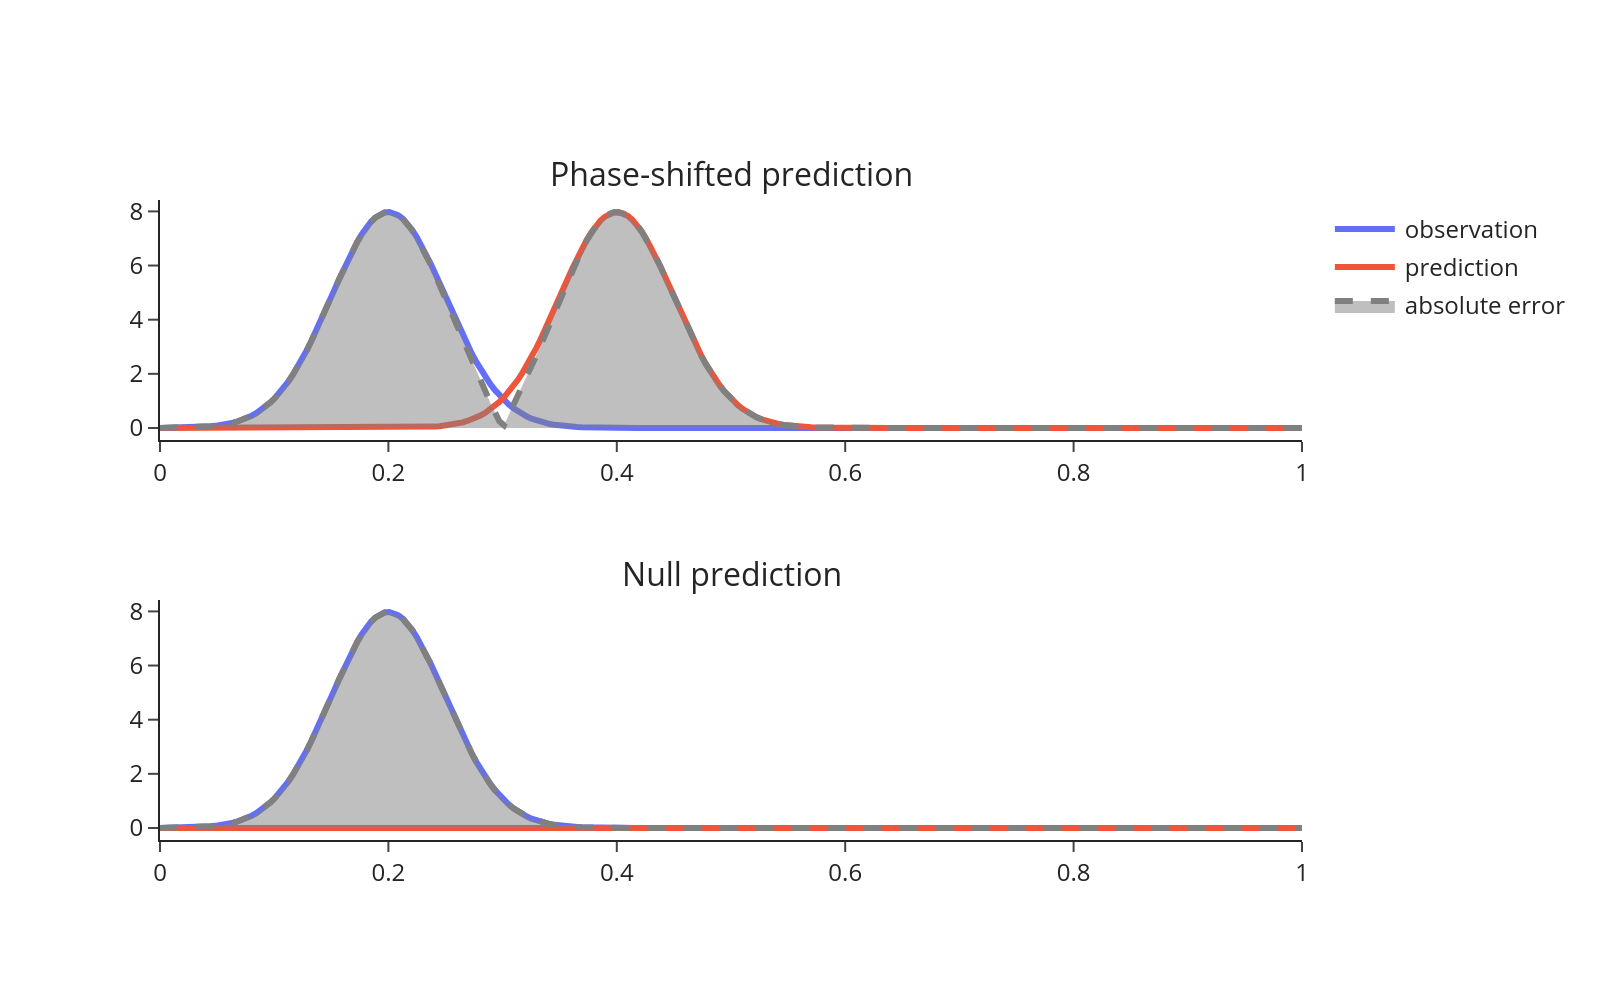
\includegraphics[width=\linewidth]{double_penalisation.png}
    \caption{Visualisation de l'effet de double pénalisation.}
    \label{fig:double_penalization_error}
\end{figure}

Un seconde limitation, concerne la nécessité pour les champs d'état et d'observation \textit{a priori} de recouvrir la solution à analyser. En effet, la mise à jour des méthodes d'assimilation de données classique consiste essentiellement à un interpolation dans l'espace des valeurs des champs, produisant ainsi une analyse encore confinée dans le support de l'état de fond et celui de l'observation. Cette remarque est d'autant plus flagrante dans le cas du filtre EnKF qui se défini justement comme combinaison des membres de l'ensemble comme décrit en Section~\ref{sec:membre}. Cette limitation est donc tout à fait en lien avec notre problème de support de discrétisation particulaire.


Pour résoudre ce problème plusieurs approches ont pu être proposées. Une première manière assez élégante est de s'inspirer de méthode de transport optimal pour définir une correction dans un espace d'interpolation plus riche et prenant en compte des déplacements~\cite{villani2009optimal,benamou_computational_2000}. Ceci passe par substitution de la norme quadratique par une norme de Wasserstein. Ainsi les travaux de thèse de Feyeux~\cite{feyeux_transport_2016} ont permis d'utiliser une distance de Wasserstein pour l'assimilation de données issues d'images. L'article de Bocquet et al. \cite{bocquet_bridging_2023} propose quand à lui une adaptation de la méthode 3D-Var au transport optimal.En particulier, son approche s'applique à des distributions d'état et d'observation de masses potentiellement différentes. Bien que les algorithmes de transport optimal ait gagnés en efficacité computationnel~\cite{cuturi_2014,peyre_computational_2019,Simsekli2018SlicedWassersteinFN}, ils restent encore difficilement applicable dans le contexte de l'assimilation de données.

Si le transport optimal permet en effet de réaliser simultanément des corrections en intensité et en position, on trouve un certain nombre de développement qui introduisent des transformations spatiales. En particulier Percival et al.~\cite{percival_department_2008} utilisent des idées en théorie du réarrangement afin d'appliquer une transformation de coordonnées. Ravela et al.~\cite{ravela_data_2007} introduisent de leur côté une variable de déplacement pour ainsi corriger indépendamment position et intensité. Cette méthode à aussi été adaptée dans une formulation multi-échelle~\cite{ying_multiscale_2019,ying_improving_2023}. Finalement, Rosenthal et al.~\cite{rosenthal_displacement_2017} présente une méthode séquentielle en deux étapes pour aligner et corriger les intensité successivement. L'objectif est alors de conserver des propriétés morphologiques de tourbillon. Pour cela, la correction est réalisée en appliquant une transformation cinématiquement admissible pour corriger la position, puis une correction d'intensité. L'avantage de cette méthode est qu'elle offre la possibilité de la coupler aux méthodes classiques d'assimilation.

C'est donc dans la continuité de ces travaux, et en particulier ceux de Rosenthal, que nous souhaitons proposer une méthode de correction de distribution particulaire des simulations sans maillage.

\section{Définition d'une méthode d'assimilation d'ensemble variationnelle non-linéaire séquentielle appliquée à la méthode vortex}~\label{sec:align_vortex}

\subsection{Transformation cinématiquement admissible de la distribution particulaire}

\subsection{Définition de l'espace de recherche}

\subsection{Réécriture du problème d'optimisation}

\section{Bilan du chapitre}

Cette section a permis de mettre en avant une méthode d'assimilation de données par correction de position. Celle-ci se veut adaptée à des discrétisations particulaires, en particulier pour la méthode vortex. Cette méthode se base sur une correction par intégration d'un champ de vitesse pour corriger l'alignement des particules. C'est une méthode variationnelle d'ensemble et de faible rang qui peut être combiné avec les filtres Part-EnKF ou Remesh-EnKF. Pour illustrer cette méthode, nous définirons et testerons les performances des différentes combinaisons de filtre dans le prochain chapitre.